\documentclass{beamer}
\usetheme{metropolis}

\usepackage[T1]{fontenc}
\let\digamma\relax
\IfFileExists{lucimatx.sty}{\usepackage[stdmathitalics=true,lucidasmallscale=true,romanfamily=bright]{lucimatx}}{\usepackage{times}}
\usepackage{../tex/varsityblueslists, ../tex/varsitybluesshortcuts, ../tex/varsitybluesmatrix}

% texlive 2020
\newlength{\cslhangindent}
\setlength{\cslhangindent}{1.5em}
\newenvironment{CSLReferences}[2]
  {}
  {\par}

\makeindex

\providecommand{\tightlist}{\setlength{\itemsep}{0pt}\setlength{\parskip}{0pt}}

% To pass between YAML and LaTeX the dollar signs are added by CII
% Syntax highlighting #22
  \usepackage{color}
  \usepackage{fancyvrb}
  \newcommand{\VerbBar}{|}
  \newcommand{\VERB}{\Verb[commandchars=\\\{\}]}
  \DefineVerbatimEnvironment{Highlighting}{Verbatim}{commandchars=\\\{\}}
  % Add ',fontsize=\small' for more characters per line
  \usepackage{framed}
  \definecolor{shadecolor}{RGB}{248,248,248}
  \newenvironment{Shaded}{\begin{snugshade}}{\end{snugshade}}
  \newcommand{\AlertTok}[1]{\textcolor[rgb]{0.94,0.16,0.16}{#1}}
  \newcommand{\AnnotationTok}[1]{\textcolor[rgb]{0.56,0.35,0.01}{\textbf{\textit{#1}}}}
  \newcommand{\AttributeTok}[1]{\textcolor[rgb]{0.77,0.63,0.00}{#1}}
  \newcommand{\BaseNTok}[1]{\textcolor[rgb]{0.00,0.00,0.81}{#1}}
  \newcommand{\BuiltInTok}[1]{#1}
  \newcommand{\CharTok}[1]{\textcolor[rgb]{0.31,0.60,0.02}{#1}}
  \newcommand{\CommentTok}[1]{\textcolor[rgb]{0.56,0.35,0.01}{\textit{#1}}}
  \newcommand{\CommentVarTok}[1]{\textcolor[rgb]{0.56,0.35,0.01}{\textbf{\textit{#1}}}}
  \newcommand{\ConstantTok}[1]{\textcolor[rgb]{0.00,0.00,0.00}{#1}}
  \newcommand{\ControlFlowTok}[1]{\textcolor[rgb]{0.13,0.29,0.53}{\textbf{#1}}}
  \newcommand{\DataTypeTok}[1]{\textcolor[rgb]{0.13,0.29,0.53}{#1}}
  \newcommand{\DecValTok}[1]{\textcolor[rgb]{0.00,0.00,0.81}{#1}}
  \newcommand{\DocumentationTok}[1]{\textcolor[rgb]{0.56,0.35,0.01}{\textbf{\textit{#1}}}}
  \newcommand{\ErrorTok}[1]{\textcolor[rgb]{0.64,0.00,0.00}{\textbf{#1}}}
  \newcommand{\ExtensionTok}[1]{#1}
  \newcommand{\FloatTok}[1]{\textcolor[rgb]{0.00,0.00,0.81}{#1}}
  \newcommand{\FunctionTok}[1]{\textcolor[rgb]{0.00,0.00,0.00}{#1}}
  \newcommand{\ImportTok}[1]{#1}
  \newcommand{\InformationTok}[1]{\textcolor[rgb]{0.56,0.35,0.01}{\textbf{\textit{#1}}}}
  \newcommand{\KeywordTok}[1]{\textcolor[rgb]{0.13,0.29,0.53}{\textbf{#1}}}
  \newcommand{\NormalTok}[1]{#1}
  \newcommand{\OperatorTok}[1]{\textcolor[rgb]{0.81,0.36,0.00}{\textbf{#1}}}
  \newcommand{\OtherTok}[1]{\textcolor[rgb]{0.56,0.35,0.01}{#1}}
  \newcommand{\PreprocessorTok}[1]{\textcolor[rgb]{0.56,0.35,0.01}{\textit{#1}}}
  \newcommand{\RegionMarkerTok}[1]{#1}
  \newcommand{\SpecialCharTok}[1]{\textcolor[rgb]{0.00,0.00,0.00}{#1}}
  \newcommand{\SpecialStringTok}[1]{\textcolor[rgb]{0.31,0.60,0.02}{#1}}
  \newcommand{\StringTok}[1]{\textcolor[rgb]{0.31,0.60,0.02}{#1}}
  \newcommand{\VariableTok}[1]{\textcolor[rgb]{0.00,0.00,0.00}{#1}}
  \newcommand{\VerbatimStringTok}[1]{\textcolor[rgb]{0.31,0.60,0.02}{#1}}
  \newcommand{\WarningTok}[1]{\textcolor[rgb]{0.56,0.35,0.01}{\textbf{\textit{#1}}}}

\author{You R. Name}
\title{My Assignment}

\makeindex

\begin{document}

% Title page frame
\begin{frame}
  \titlepage
\end{frame}

\begin{frame}
\end{frame}

\begin{frame}{R Markdown Basics}
\protect\hypertarget{rmd-basics}{}
Here is a brief introduction into using \emph{R Markdown}.
\emph{Markdown} is a simple formatting syntax for authoring HTML, PDF,
and MS Word documents. \emph{R Markdown} provides the flexibility of
\emph{Markdown} with the implementation of \textbf{R} input and output.
For more details on using \emph{R Markdown} see
\url{https://rmarkdown.rstudio.com}.
\end{frame}

\begin{frame}
Be careful with your spacing in \emph{Markdown} documents. While
whitespace largely is ignored, it does at times give \emph{Markdown}
signals as to how to proceed. As a habit, try to keep everything left
aligned whenever possible, especially as you type a new paragraph. In
other words, there is no need to indent basic text in the Rmd document
(in fact, it might cause your text to do funny things if you do).
\end{frame}

\begin{frame}
\begin{block}{Lists}
\protect\hypertarget{lists}{}
It's easy to create a list. It can be unordered like

\begin{itemize}
\tightlist
\item
  Item 1
\item
  Item 2
\end{itemize}

or it can be ordered like

\begin{enumerate}
\tightlist
\item
  Item 1
\item
  Item 2
\end{enumerate}
\end{block}
\end{frame}

\begin{frame}
Notice that I intentionally mislabeled Item 2 as number 4.
\emph{Markdown} automatically figures this out! You can put any numbers
in the list and it will create the list. Check it out below.

To create a sublist, just indent the values a bit (at least four spaces
or a tab). (Here's one case where indentation is key!)

\begin{enumerate}
\tightlist
\item
  Item 1
\item
  Item 2
\item
  Item 3

  \begin{itemize}
  \tightlist
  \item
    Item 3a
  \item
    Item 3b
  \end{itemize}
\end{enumerate}
\end{frame}

\begin{frame}
\begin{block}{Line breaks}
\protect\hypertarget{line-breaks}{}
Make sure to add white space between lines if you'd like to start a new
paragraph. Look at what happens below in the outputted document if you
don't:

Here is the first sentence. Here is another sentence. Here is the last
sentence to end the paragraph.

This should be a new paragraph.
\end{block}
\end{frame}

\begin{frame}
\emph{Now for the correct way:}

Here is the first sentence. Here is another sentence. Here is the last
sentence to end the paragraph.

This should be a new paragraph.
\end{frame}

\begin{frame}
\begin{block}{R chunks}
\protect\hypertarget{r-chunks}{}
When you click the \textbf{Knit} button above a document will be
generated that includes both content as well as the output of any
embedded \textbf{R} code chunks within the document.
\end{block}
\end{frame}

\begin{frame}[fragile]
You can embed an \textbf{R} code chunk like this (\texttt{mtcars} is a
built-in \textbf{R} dataset):

\begin{Shaded}
\begin{Highlighting}[]
\FunctionTok{summary}\NormalTok{(mtcars)}
\end{Highlighting}
\end{Shaded}

\begin{verbatim}
##       mpg             cyl             disp             hp       
##  Min.   :10.40   Min.   :4.000   Min.   : 71.1   Min.   : 52.0  
##  1st Qu.:15.43   1st Qu.:4.000   1st Qu.:120.8   1st Qu.: 96.5  
##  Median :19.20   Median :6.000   Median :196.3   Median :123.0  
##  Mean   :20.09   Mean   :6.188   Mean   :230.7   Mean   :146.7  
##  3rd Qu.:22.80   3rd Qu.:8.000   3rd Qu.:326.0   3rd Qu.:180.0  
##  Max.   :33.90   Max.   :8.000   Max.   :472.0   Max.   :335.0  
##       drat             wt             qsec             vs        
##  Min.   :2.760   Min.   :1.513   Min.   :14.50   Min.   :0.0000  
##  1st Qu.:3.080   1st Qu.:2.581   1st Qu.:16.89   1st Qu.:0.0000  
##  Median :3.695   Median :3.325   Median :17.71   Median :0.0000  
##  Mean   :3.597   Mean   :3.217   Mean   :17.85   Mean   :0.4375  
##  3rd Qu.:3.920   3rd Qu.:3.610   3rd Qu.:18.90   3rd Qu.:1.0000  
##  Max.   :4.930   Max.   :5.424   Max.   :22.90   Max.   :1.0000  
##        am              gear            carb      
##  Min.   :0.0000   Min.   :3.000   Min.   :1.000  
##  1st Qu.:0.0000   1st Qu.:3.000   1st Qu.:2.000  
##  Median :0.0000   Median :4.000   Median :2.000  
##  Mean   :0.4062   Mean   :3.688   Mean   :2.812  
##  3rd Qu.:1.0000   3rd Qu.:4.000   3rd Qu.:4.000  
##  Max.   :1.0000   Max.   :5.000   Max.   :8.000
\end{verbatim}
\end{frame}

\begin{frame}[fragile]
\begin{Shaded}
\begin{Highlighting}[]
\FunctionTok{hist}\NormalTok{(mtcars}\SpecialCharTok{$}\NormalTok{wt)}
\end{Highlighting}
\end{Shaded}

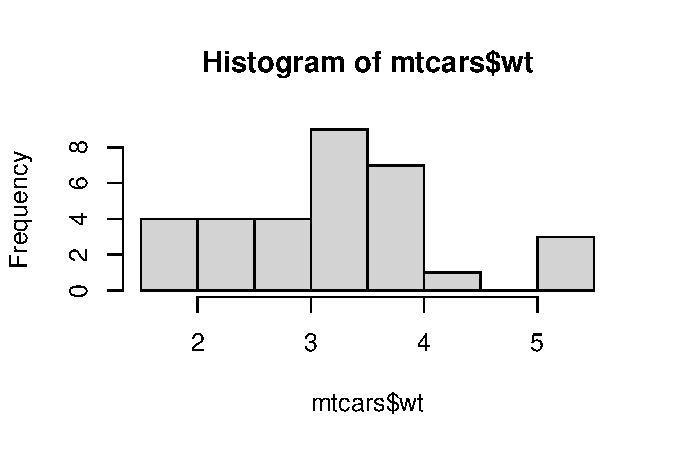
\includegraphics{presentation1_files/figure-beamer/mtcars2-1.pdf}
\end{frame}

\begin{frame}[fragile]
\begin{block}{Inline code}
\protect\hypertarget{inline-code}{}
If you'd like to put the results of your analysis directly into your
discussion, add inline code like this:

\begin{quote}
The \texttt{cos} of \(2 \pi\) is 1.
\end{quote}

Another example would be the direct calculation of the standard
deviation:

\begin{quote}
The standard deviation of \texttt{speed} in \texttt{cars} is 5.2876444.
\end{quote}
\end{block}
\end{frame}

\begin{frame}[fragile]
One last neat feature is the use of the \texttt{ifelse} conditional
statement which can be used to output text depending on the result of an
\textbf{R} calculation:

\begin{quote}
The standard deviation is less than 6.
\end{quote}

Note the use of \texttt{\textgreater{}} here, which signifies a
quotation environment that will be indented.
\end{frame}

\begin{frame}[fragile]
As you see with \texttt{\$2\ \textbackslash{}pi\$} above, mathematics
can be added by surrounding the mathematical text with dollar signs.
More examples of this are in
\protect\hyperlink{mathematical-equations}{Mathematical equations}.
\end{frame}

\begin{frame}{Mathematical equations}
\protect\hypertarget{mathematical-equations}{}
\TeX~is the best way to typeset mathematics. Donald Knuth designed
\TeX~when he got frustrated at how long it was taking the typesetters to
finish his book, which contained a lot of mathematics.

One nice feature of \emph{R Markdown} is its ability to read LaTeX code
directly.
\end{frame}

\begin{frame}
\begin{block}{A quick example of \emph{some} of the package's shortcuts}
\protect\hypertarget{a-quick-example-of-some-of-the-packages-shortcuts}{}
Let \(K\) be a field of
\dfn{scalars}\index{field!scalar}\index{scalar}---usually either the
real numbers \(\R\) or the complex numbers \(\mathbb C\), or
occasionally the rationals \(\mathbb Q\). A \idfn{vector space} over
\(K\) is a set \(V\) of \dfn{vectors}\index{vector} equipped with two
operations, vector addition \((x,y)\mapsto x+y\), and scalar
multiplication \((\alpha,x)\mapsto \alpha x\), where \(x,y\in V\) and
\(\alpha\in K\).
\end{block}
\end{frame}

\begin{frame}
The operations satisfy:

\begin{description}
\item[V.1] $x+y=y+x$
\item[V.2] $(x+y)+z=x+(y+z)$
\item[V.3] There is a vector $0$, satisfying $x+0=x$ for every vector $x$.
\item[V.4] $x+(-1)x=0$
\item[V.5] $\alpha(\beta x)=(\alpha \beta)x$
\item[V.6] $1x=x$
\item[V.7] $\alpha(x+y)=(\alpha x)+(\alpha y)$
\item[V.8] $(\alpha+\beta)x=(\alpha x)+(\beta x)$
\end{description}
\end{frame}

\begin{frame}
\begin{block}{Statistical notation}
\protect\hypertarget{statistical-notation}{}
\begin{itemize}
\tightlist
\item
  Algebra and semi-algebra: \(\A,\S\)
\item
  Sigma field: \(\F\)
\item
  Set of probability measures: \(\prob\), \(\prob{X}\), \(\prob{A}\),
  etc
\item
  Probability of \(x\): \(\P(X = x)\)
\item
  Different thetas: \(\thetah, \thetat\)
\item
  Convergence in probability: \(\thetah \probconv \theta\)
\item
  Union and intersection:
  \(\infunion, \infintersection, \union{a}{b}, \intersection{a}{b}\)
\item
  Normal distributions: \(\normalstd, \normal{\mu}{\sigma^2}\)
\item
  Measurable and probability space: \(\mespace, \prspace\)
\end{itemize}
\end{block}
\end{frame}

\begin{frame}
\begin{block}{Calculus notation}
\protect\hypertarget{calculus-notation}{}
Many shortcuts for derivatives. Let \(\fn1\), then
\[\dfx, \dfy, \dfi, \dfj\] \[\dFx, \dFy, \dFi, \dFj\] Same for \(g()\)
which is \(\gn1\) \[\dgx, \dgy, \dgi, \dgj\]

Now let \(f\) be a \(\C^2\) function \[
\ddfyx, \ddfxy, \ddfx, \ddfy, \ddfij, \ddfji, \ldots, \dfij
\]
\end{block}
\end{frame}

\begin{frame}
You can also have \(\fgn1\) and \(\fgnm\).

In general, you can write \[
\prd{f}{x}
\] or more general
\[\diff{L}{}{\beta}{} \text{ or } \diffat{L}{}{\beta}{}{\hat\beta_{\lambda}}\]
which is more flexible because it allows
\[\diffat{L}{2}{\beta}{3}{\hat\beta_{\lambda}}\]
\end{frame}

\begin{frame}[fragile]
\begin{block}{Matrices}
\protect\hypertarget{matrices}{}
You can also type matrices with relative efficiency. Here are some
simple examples of use, and of course you can use \LaTeX default
commands.

Start by replacing
\texttt{\textbackslash{}left{[}\textbackslash{}begin\{array\}\{...\}} by
\texttt{\textbackslash{}vbmatrix\{}. Note that there is no column
specifier. You can make as many columns as you like, but they will all
be centered. To finish, instead of
\texttt{\textbackslash{}end\{array\}\textbackslash{}right{]}}, just type
\texttt{\}}. Like this:

\[
\vbmatrix{\mbox{indices}&1&2&3&4\\
1&M_{1,1}&M_{1,2}&M_{1,3}&M_{1,4}\\
2&M_{2,1}&M_{2,2}&M_{2,3}&M_{2,4}
}
\]
\end{block}
\end{frame}

\begin{frame}[fragile]
You can also add a vertical rule and if you don't like all the
horizontal space around the vertical rule, you can get rid of it using
plain TEX's \texttt{\textbackslash{}omit} command.

\[
\vbmatrix{\mbox{indices}&
1&2&\omit\vrule&3&4\\
1&M_{1,1}&M_{1,2}&\omit\vrule&
M_{1,3}&M_{1,4}\\
2&M_{2,1}&M_{2,2}&\omit\vrule&
M_{2,3}&M_{2,4}}
\]
\end{frame}

\begin{frame}[fragile]
If you think the vertical rule in the first row is too tall, you can
shorten it using plain TEX's \texttt{height} command.

\[
\vbmatrix{\mbox{indices}&
1&2&\omit\vrule height 1ex&3&4\\
1&M_{1,1}&M_{1,2}&\omit\vrule&
M_{1,3}&M_{1,4}\\
2&M_{2,1}&M_{2,2}&\omit\vrule&
M_{2,3}&M_{2,4}}
\]
\end{frame}

\begin{frame}
Horizontal lines works as you might expect.

\[
\vbmatrix{\mbox{indices}&
1&2&\vrule&3&4\\
1&M_{1,1}&M_{1,2}&\vrule&
M_{1,3}&M_{1,4}\\\hline
2&M_{2,1}&M_{2,2}&\vrule&
M_{2,3}&M_{2,4}
}
\]
\end{frame}

\begin{frame}[fragile]
Notice how the \texttt{\textbackslash{}hline} cuts across all the
columns, but it doesn't connect to the closing bracket. I am not sure I
like this behavior, but you can use \texttt{\textbackslash{}cline}.

\[
\vbmatrix{\mbox{indices}&1&2&
\vrule&3&4\\
1&M_{1,1}&M_{1,2}&\vrule&M_{1,3}&
M_{1,4}\\\cline{1-1} \cline{2-6}
2&M_{2,1}&M_{2,2}&\vrule&M_{2,3}&
M_{2,4}}
\]

\[
\vbmatrix{\mbox{indices}&1&2&
\vrule&3&4\\
1&M_{1,1}&M_{1,2}&\vrule&M_{1,3}&
M_{1,4}\\\cline{2-6}
2&M_{2,1}&M_{2,2}&\vrule&
M_{2,3}&M_{2,4}
}
\]
\end{frame}

\begin{frame}[fragile]
Here's a more complex example that summarises the previous steps.

\[
\vbmatrix{\text{indices}&
(1\cdot11)&(1\cdot12)&(1\cdot22)&
\vrule&
(2\cdot11)&(2\cdot12)&(2\cdot22)\\
%
(1)&\lambda(1)^2&2\lambda(1)\lambda(2)&\lambda(2)^2&\vrule&0&0&0\\
3
(2)&0&0&0&\vrule&\lambda(1)^2&2\lambda(1)\lambda(2)&\lambda(2)^2\\
\hline
(111)&3&0&0&\vrule&0&0&0\\
(112)&0&2&0&\vrule&1&0&0\\
(122)&0&0&1&\vrule&0&2&0\\
(222)&0&0&0&\vrule&0&0&3}
\]

where \texttt{\textbackslash{}text\{\}} is defined in the amstext
\LaTeX package.
\end{frame}

\begin{frame}[fragile]
\begin{block}{Changing delimiters}
\protect\hypertarget{changing-delimiters}{}
The varsitybluesmatrix package defines four style parameters that can be
used to change the appearance of the array. The first two are
\texttt{\textbackslash{}vbldelim} and \texttt{\textbackslash{}vbrdelim},
the left and right delimiters. By default they are \texttt{{[}} and
\texttt{{]}} but you can change them like this:

\[
\renewcommand{\vbldelim}{\{}
\renewcommand{\vbrdelim}{.}
\vbmatrix{\mbox{indices}&1&2&
\vrule&3&4\\
1&M_{1,1}&M_{1,2}&\vrule&M_{1,3}&
M_{1,4}\\\cline{2-6}
2&M_{2,1}&M_{2,2}&\vrule&
M_{2,3}&M_{2,4}
}
\]
\end{block}
\end{frame}

\begin{frame}
Another option:

\[
\renewcommand{\vbldelim}{\langle}
\renewcommand{\vbrdelim}{|} 
\vbmatrix{\mbox{indices}&1&2&
\vrule&3&4\\
1&M_{1,1}&M_{1,2}&\vrule&M_{1,3}&
M_{1,4}\\\cline{2-6}
2&M_{2,1}&M_{2,2}&\vrule&
M_{2,3}&M_{2,4}
}
\]
\end{frame}

\begin{frame}
Yet another option:

\[
\renewcommand{\vbldelim}{(}
\renewcommand{\vbrdelim}{)} 
\vbmatrix{\mbox{indices}&1&2&
\vrule&3&4\\
1&M_{1,1}&M_{1,2}&\vrule&M_{1,3}&
M_{1,4}\\\cline{2-6}
2&M_{2,1}&M_{2,2}&\vrule&
M_{2,3}&M_{2,4}
}
\]
\end{frame}

\begin{frame}[fragile]
\begin{block}{Changing the border row and column style}
\protect\hypertarget{changing-the-border-row-and-column-style}{}
You can change the style of the border row and column column entries by
redefining \texttt{\textbackslash{}vbrowstyle} and
\texttt{\textbackslash{}vbcolstyle}, which are by default set to
\texttt{\textbackslash{}scriptstyle}. You could, for instance, say
\texttt{\textbackslash{}renewcommand\{\textbackslash{}vbrowstyle\}\{\textbackslash{}relax\}}
to typeset the first row as usual. By the way, the upper left corner is
governed by the column style. You can always use an
\texttt{\textbackslash{}mbox\{\}} to change the style of any particular
entry.
\end{block}
\end{frame}

\begin{frame}[fragile]
\begin{block}{Changing spacing}
\protect\hypertarget{changing-spacing}{}
Besides changing the delimiters, you can also change the space inserted
after the first row and after the first column. These are governed by
the lengths \texttt{\textbackslash{}vbrowsep} and
\texttt{\textbackslash{}vbcolsep}. By default they are \texttt{0pt} and
\texttt{.5\textbackslash{}arraycolsep}, respectively.

\[
\setlength{\vbrowsep}{10pt}
\setlength{\vbcolsep}{10pt}
\vbmatrix{\mbox{indices}&1&2&
\vrule&3&4\\
1&M_{1,1}&M_{1,2}&\vrule&M_{1,3}&
M_{1,4}\\\cline{2-6}
2&M_{2,1}&M_{2,2}&\vrule&
M_{2,3}&M_{2,4}
}
\]
\end{block}
\end{frame}

\begin{frame}[fragile]{Additional resources}
\protect\hypertarget{additional-resources}{}
\begin{itemize}
\tightlist
\item
  \href{https://github.com/adam-p/markdown-here/wiki/Markdown-Cheatsheet}{\emph{Markdown}
  Cheatsheet}
\item
  \href{https://www.rstudio.com/wp-content/uploads/2015/03/rmarkdown-reference.pdf}{\emph{R
  Markdown} Reference Guide}
\item
  \href{https://github.com/rstudio/cheatsheets/raw/master/rmarkdown-2.0.pdf}{\emph{R
  Markdown} Cheatsheet}
\item
  \href{https://github.com/rstudio/cheatsheets/raw/master/rstudio-ide.pdf}{\emph{RStudio
  IDE} Cheatsheet}
\item
  \href{https://rstudio.com/products/rstudio/}{\emph{RStudio IDE}
  Official website}
\item
  \href{https://cran.rstudio.com/web/packages/dplyr/vignettes/dplyr.html}{Introduction
  to \texttt{dplyr}}
\item
  \href{https://ggplot2.tidyverse.org/}{\texttt{ggplot2} Documentation}
\item
  \href{https://github.com/rstudio/cheatsheets/raw/master/data-visualization-2.1.pdf}{\texttt{ggplot2}
  Cheatsheet}
\end{itemize}
\end{frame}

\begin{frame}{References}
\protect\hypertarget{references}{}
\markboth{References}{References}

\noindent

\hypertarget{refs}{}
\begin{CSLReferences}{1}{0}
\leavevmode\hypertarget{ref-angel2001}{}%
Angel, Edward. \emph{Batch-File Computer Graphics : A Bottom-up Approach
with QuickTime}. Boston, MA: Wesley Addison Longman, 2001.

\leavevmode\hypertarget{ref-angel2000}{}%
---------. \emph{Interactive Computer Graphics : A Top-down Approach
with OpenGL}. Boston, MA: Addison Wesley Longman, 2000.

\leavevmode\hypertarget{ref-angel2002a}{}%
---------. \emph{Test Second Book by Angel}. Boston, MA: Wesley Addison
Longman, 2001.

\end{CSLReferences}
\end{frame}

\end{document}
